\documentclass[letterpaper,10pt]{article}

\usepackage{titling}
\usepackage{listings}
\usepackage{url}
\usepackage{setspace}
\usepackage{subfig}
\usepackage{sectsty}
\usepackage{pdfpages}
\usepackage{colortbl}
\usepackage{multirow}
\usepackage{multicol}
\usepackage{relsize}
\usepackage{amsmath}
\usepackage{fancyvrb}
\usepackage[yyyymmdd]{datetime}
\usepackage{amsmath,amssymb,amsthm,graphicx,xspace}
\usepackage[titlenotnumbered,noend,noline]{algorithm2e}
\usepackage[compact]{titlesec}
\usepackage{XCharter}
\usepackage[T1]{fontenc}
\usepackage{tikz}
\usetikzlibrary{arrows,automata,shapes,trees,matrix,chains,scopes,positioning,calc}
\tikzstyle{block} = [rectangle, draw, fill=blue!20, 
    text width=2.5em, text centered, rounded corners, minimum height=2em]
\tikzstyle{bw} = [rectangle, draw, fill=blue!20, 
    text width=4em, text centered, rounded corners, minimum height=2em]

\definecolor{namerow}{cmyk}{.40,.40,.40,.40}
\definecolor{namecol}{cmyk}{.40,.40,.40,.40}
\renewcommand{\dateseparator}{-}


\let\LaTeXtitle\title
\renewcommand{\title}[1]{\LaTeXtitle{\textsf{#1}}}


\newcommand{\handout}[5]{
  \noindent
  \begin{center}
  \framebox{
    \vbox{
      \hbox to 5.78in { {\bf ECE252: Systems Programming and Concurrency } \hfill #2 }
      \vspace{4mm}
      \hbox to 5.78in { {\Large \hfill #4  \hfill} }
      \vspace{2mm}
      \hbox to 5.78in { {\em #3 \hfill \today } }
    }
  }
  \end{center}
  \vspace*{4mm}
}

\newcommand{\lecture}[3]{\handout{#1}{#2}{#3}{Lecture #1}}{
\newcommand{\tuple}[1]{\ensuremath{\left\langle #1 \right\rangle}\xspace}

\addtolength{\oddsidemargin}{-1.000in}
\addtolength{\evensidemargin}{-0.500in}
\addtolength{\textwidth}{2.0in}
\addtolength{\topmargin}{-1.000in}
\addtolength{\textheight}{1.75in}
\addtolength{\parskip}{\baselineskip}
\setlength{\parindent}{0in}
\renewcommand{\baselinestretch}{1.5}
\newcommand{\term}{Spring 2019}

\singlespace


\begin{document}

\lecture{ 12 --- Semaphores }{\term}{Jeff Zarnett}

\section*{Mutual Exclusion through Messages}

The earlier definition of mutual exclusion said only that one thread may be in the critical section at a time. This is the minimum, but there are additional desirable properties that will be used to evaluate any solution~\cite{osi}:
\begin{enumerate}
	\item Mutual exclusion must apply (this criterion eliminated most of the flag examples earlier).
	\item A thread that halts outside the critical section must not interfere with other threads (the strict alternation routine, even if implemented with Test-and-Set, would fail on this criterion).
	\item It must not be possible for a thread requiring access to a critical section to be delayed indefinitely (the situation where all threads get stuck, each thinking another is in the critical section, would fail this criterion).
	\item When no thread is in the critical section, a thread that requests access should be allowed to enter right away (no unnecessary waiting).
	\item No assumptions are made about what the threads will do or the number of processors in the system (so it should be a general solution, not a special case).
	\item A thread remains inside the critical section for a finite time only (this is more of an assumption than a criterion, but our solution must provide a way to indicate the thread has left the critical section).
\end{enumerate}

Recall from earlier the example of the employees Alice and Bob who worked at the Springfield Nuclear Power Plant in Sector 7G.  Suppose there is a third employee at the power plant, Charlie, who works on the day shift at the same time as Alice. Safety rules say that at least one of them has to monitor the safety of the reactor at all times and therefore they cannot both take lunch at the same time. If we cannot predict when lunch begins or how long it will last, how can Alice and Charlie co-ordinate to make sure they don't take lunch at the same time?

A possible solution: before Alice gets up from her desk to go for lunch, she calls Charlie. If he does answer, she may proceed. If Charlie does not answer, Alice will know he is not at his desk and she cannot leave at the moment. She can call again, constantly, until she reaches Charlie (busy-waiting), but this ties up a phone line nonstop and is effort intensive for Alice. If she doesn't want to do that, at this point she has two options: one is to simply wait some period of time (perhaps 15 minutes) and call again in the hopes that at that time Charlie will be back from lunch. A better approach would be for Alice to leave a message in Charlie's voice mail box, asking him to call her back when he has finished lunch. Then Alice can go about her work until she gets a call from Charlie and as soon as that happens, she may step out for lunch.

Busy waiting has already been found inadequate as a solution. It wastes CPU time that another process or thread could be putting to productive use. The approach of ``wait 15 minutes and try again'' might be adequate for Alice as a human, but for the computer it is not ideal. If thread $B$ is in the critical section when $A$ tries to get in, and $A$ then sleeps for 2000~ms before trying again, this at least means $A$ is not wasting CPU cycles while it tries futilely to ask ``is it my turn now? Now? Now? Now? Now? Now?'', but if $B$ is finished after 20 ms, then thread $A$ waits unnecessarily for 1980~ms. 

What we want is something that resembles the call-when-finished semantics of Alice leaving a message and Charlie calling her back. That solution is called the Semaphore.

\section*{Semaphore}
A semaphore, outside of the context of computing, is a system of signals used for communication. Before ships had radios, when two friendly ships were in visual range, they would communicate with one another through flag semaphores, which is a fancy way of saying each ship had someone holding certain flags in a specific position. Thus the two ships could co-ordinate at a distance, even if the distance was limited to visual range. This worked dramatically better than many alternatives (e.g., shouting).

The computer semaphore was invented in 1965 by Edsger Dijkstra, a brilliant Dutch computer scientist who is sometimes maligned in textbooks as being eccentric or unusual.  He described a data structure that can be used to solve synchronization problems via messages in~\cite{semaphores}. Although the version we use now is not exactly the same as the original description, even 50 years later, the core idea is unchanged.

We will begin with the \textit{binary semaphore}: this is a variable that has two values, 0 and 1. It can be initialized to 0 or to 1. The semaphore has two operations: \texttt{wait} and \texttt{signal}. In the original paper, \texttt{wait} was called \texttt{P} and \texttt{signal} was called \texttt{V}, but the names in common usage have become a little more descriptive. Mind you, if you can read/write Dutch as I can, the names make some sense: \texttt{P} is short for \textit{proberen}, ``to test'', and \texttt{V} is short for \textit{verhogen}, ``to raise'' or ``to increment''. But, for historical reasons as much as any other, the traditional lingua franca of computers is English, so the English names have tended to dominate. Furthermore, \texttt{signal} is also called \texttt{post} in many textbooks.

The \texttt{wait} operation on the semaphore is how a program tries to enter the critical section. When \texttt{wait} is called, if the semaphore value is 1, set it to 0 and this thread may enter the critical section and continue. If the semaphore is 0, some other thread is in the critical section and the current thread must \textit{wait} its turn. The thread that called \texttt{wait} will be blocked by the operating system, just as if it asked for memory or a disk operation. This is sometimes referred to as decrementing the semaphore (because the value changes from 1 to 0).

The \texttt{signal} operation is how a program \textit{signals}, or indicates, it is finished with the critical section. When this is called, if the semaphore is 1, do nothing; if the semaphore is 0 and there is a task blocked awaiting that semaphore, that task may be unblocked; else set the semaphore to 1. This is also sometimes called incrementing the semaphore.

If this is still confusing, consider the following analogy. Suppose you like coffee, and going to a particular coffee shop because there you can get your drink exactly the way you like it: half caf, no whip, extra hot, extra foam, two shot, soy milk latte\footnote{For the record, the author drinks tea, black.}. After this delightful beverage it may be the case that you need to use the washroom. The washroom is locked at such places, so to get in you will need the key, which is available by asking one of the employees. If nobody is currently in the washroom, you will get the key and can proceed. If it is currently occupied, you will have to wait. When the key is returned, if anyone is waiting, the employee will give the key to the first person in line for the washroom; otherwise he or she will put the key away behind the counter.

Observe that the operating system is needed to make this work: if thread $A$ attempts to wait on a semaphore that some other thread already has, it will be blocked and the operating system knows not to schedule it to run until it is unblocked. When thread $B$ is finished and signals the semaphore it is holding, that will unblock $A$ and allow it to run again.

Note also that the semaphore does not provide any facility to ``check''the current value. Thus a thread does not know in advance if it will block when it waits on the semaphore. It can only wait and may be blocked or may proceed directly into the critical section if there is no other thread in there at the moment.

When a thread signals a semaphore, it likewise does not know if any other thread(s) are waiting on that semaphore. There is no facility to check this, either. When thread $A$ signals a semaphore, if another thread $B$ is waiting, $B$ will be unblocked and either thread $A$ or thread $B$ may continue execution (or both, if it is a SMP system), or another unrelated thread may be the one to continue execution. We have no way of knowing.

On the subject of observation, note that nothing about the semaphore as so defined protects against certain ``bad'' behaviour. Suppose thread $C$ would like to enter the critical section. The programmer of this task is malicious as well as impatient: ``my task is FAR too important to wait for those other processes and threads,'' he says, as he implements his code such that before he waits on the semaphore, he signals it. Even though $A$ or $B$ might be in the critical section, the semaphore gets signalled so he is more or less certain that his program will now get to enter the critical section. It's not foolproof: if there are other threads waiting, they might get woken up to proceed instead of $C$; much depends on the scheduler. Nevertheless, this is really bad: one process can wreak all kinds of havoc by letting another process into the critical section. Though the example here makes the author of thread $C$ a scheming villain (because the example is funnier that way), such a situation may occur without malicious intent if it is simply the result of a programming error.

The problem identified in the previous paragraph is usually solved by supplementing the basic binary semaphore. A data structure called a \textit{mutex} (from \textbf{mut}ual \textbf{ex}clusion) is a binary semaphore with an additional rule enforced: only the thread that has called \texttt{wait} may \texttt{signal} that semaphore. This adds a small amount of extra bookkeeping to the semaphore, but this is a reasonable price to pay.

\subsection*{Example: Linked List Integrity}
We will now examine a situation where a semaphore helps to prevent a synchronization error. This example comes from~\cite{mte241}. Imagine we have a shared linked list defined as:

\begin{verbatim}
typedef struct single_node {
  void *element;
  struct single_node *next;
} single_node_t;

typedef struct single_list {
  single_node_t *head;
  single_node_t *tail;
  int size;
} single_list_t;


void single_list_init( single_list_t *list ) {
  list->head = NULL;
  list->tail = NULL;
  list->size = 0;
}

bool push_front( single_list_t *list, void *obj ) {
  single_node_t *tmp = (single_node_t *) malloc( sizeof( single_node_t ) );
  
  if ( tmp == NULL ) {
    return false;
  }
  
  tmp->element = obj;
  tmp->next = list->head;
  list->head = tmp;

  if ( list->size == 0 ) {
     list->tail = tmp;
  }
  
   ++( list->size );
   return true;
}
\end{verbatim}

If only one thread access this data structure, we do not have a problem, but it was a shared linked list. Suppose a thread runs and tries to add an element $A$ to the list using the \texttt{push\_front} function. Right before the increment of the \texttt{size} field takes place there is a process switch. At this point, the new node has been allocated and initialized, the pointers of \texttt{head} and \texttt{tail} have been updated, but \texttt{size} is 0. 

\begin{center}
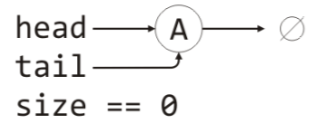
\includegraphics[width=0.25\textwidth]{images/linkedlist1.png}\\
The linked list at the time of the thread switch~\cite{mte241}.
\end{center}

Now, the second thread executes and wants to add $B$ to the linked list. In the conditional statement, \texttt{list->size == 0} evaluates to true. Thus, the \texttt{tail} pointer is updated.

\begin{center}
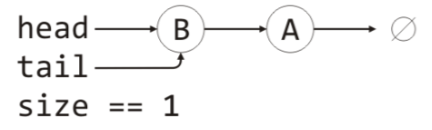
\includegraphics[width=0.35\textwidth]{images/linkedlist2.png}\\
The linked list after the second thread adds $B$~\cite{mte241}.
\end{center}

When the first thread gets to run again, it will resume where it left off: it increments the \texttt{size} integer, leaving the final state: \texttt{head} and \texttt{tail} both point to element $B$, even though there is element $A$ in the list.

\begin{center}
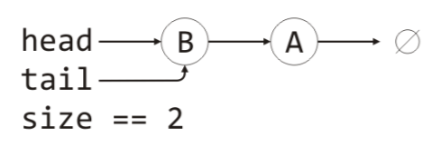
\includegraphics[width=0.35\textwidth]{images/linkedlist3.png}\\
The linked list after the first thread resumes~\cite{mte241}.
\end{center}

This is an \textit{inconsistent state}: the linked list has two elements in it but the \texttt{tail} pointer is wrong. An attempt to remove an element from the list will reveal the problem, which can manifest in a few ways, depending on how the removal routine is implemented. If we try to remove the front element we might check that \texttt{head} and \texttt{tail} are equal, and that may give the mistaken impression that $B$ is the last element in the list, so we ``lose'' $A$ and it becomes a memory leak. Or perhaps the \texttt{head} pointer will be updated but \texttt{tail} will still point to $B$ even after it has been freed, which can result in a segmentation fault or invalid access.

\subsection*{Binary Semaphore Syntax}
The linked list problem just discussed can be solved easily if a semaphore is employed. The syntax we will use is as follows:

\texttt{semaphore\_init( semaphore\_t *sem, int i )}\\
Initialize the semaphore to \texttt{i} (can be 0 or 1).

\texttt{semaphore\_wait( semaphore\_t *sem )}\\
Wait on a semaphore.

\texttt{semaphore\_signal( semaphore\_t *sem)}\\
If the semaphore is 1, do nothing.\\
If the semaphore is 0 and there is at least one task blocked on this semaphore, unblock it; otherwise set the semaphore to 1.

\subsection*{Applying the Semaphore to the Linked List}

Now that we have the appropriate syntax we can apply it to the linked list example from this section. We will add to the linked list structure (\texttt{struct single\_list}) a semaphore: \texttt{semaphore\_t mutex;}. In the initialization routine, we need to call the initialization method: \texttt{semaphore\_init( \&( list->mutex ), 0 );}

Finally, the \texttt{semaphore\_wait} and \texttt{semaphore\_signal} operations need to be added to \texttt{push\_front} at the start and end of the critical section, respectively. Recall from earlier that we want the critical section to be as small as it can be. Putting it all together:

\begin{verbatim}
typedef struct single_node {
  void *element;
  struct single_node *next;
} single_node_t;

typedef struct single_list {
  single_node_t *head;
  single_node_t *tail;
  int size;
  semaphore_t mutex;
} single_list_t;


void single_list_init( single_list_t *list ) {
  list->head = NULL;
  list->tail = NULL;
  list->size = 0;

  semaphore_init( &( list->mutex ), 0 );
}

bool push_front( single_list_t *list, void *obj ) {
  single_node_t *tmp = (single_node_t *) malloc( sizeof( single_node_t ) );
  
  if ( tmp == NULL ) {
    return false;
  }
  
  tmp->element = obj;
  
  semaphore_wait( &( list->mutex ) ); {
  
    tmp->next = list->head;
    list->head = tmp;

    if ( list->size == 0 ) {
       list->tail = tmp;
    }
    ++( list->size );
  
  } semaphore_signal( &( list->mutex ) );
  
  
  return true;
}
\end{verbatim}

Strictly speaking, the braces (\{ \}) to enclose the critical region (between the wait and signal operations) are not necessary. This is just a use of C syntax to make it more obvious what the critical region is and to make it harder to make a mistake.

The critical section here just encloses the modification of the shared linked list. In theory one might put the wait and signal operations at the start and end of the entire function, respectively. This is, however, suboptimal: it forces unnecessary waiting. In this specific example, including the call to \texttt{malloc} is especially bad; the memory allocation itself can block if insufficient memory is available. Thus the process currently in the critical section is blocked and that means no other thread can enter the critical section. This might result in the system getting totally stuck~\cite{mte241}.

\subsection*{Counting Semaphores}
Binary semaphores are useful, and we can generalize this concept to what is known as a \textit{counting} or \textit{general} semaphore. Instead of having only the values 0 and 1, the setup routine for the counting semaphore allows the choice of an integer value and this is the maximum value. A thread that waits on that semaphore will decrement the integer by 1; a thread that signals on the semaphore will increment the integer by 1. If a thread attempts to wait on a semaphore and the decrement operation makes the integer value zero or negative, the calling thread is blocked. If, however, the semaphore is, for example, initialized with 5 and the current value is 2, a thread that waits on that general semaphore will not be blocked.

In some operating systems there is no distinction between binary and counting semaphores; the binary semaphore behaviour is achieved by creating a counting semaphore that will permit only one thread into the critical section at a time. 

The general semaphore initialization function signature now takes an extra parameter, \texttt{n}, to show the maximum value of the semaphore.

\texttt{semaphore\_init( semaphore\_t *sem, int i, int n )}\\
Initialize the semaphore to \texttt{i} with a maximum value of \texttt{n}.


\bibliographystyle{alphaurl}
\bibliography{252}


\end{document}